% displayname : Ondes acoustiques dans les fluides
\documentclass[12pt,fancy]{cours}
\Chapit{6}{2}
\begin{document}
\maketitre[***]{
	Nous étudions dans ce chapitre un phénomène propagatif toujours non dispersif, celui de la propagation d'une onde acoustique, qui est une onde mécanique dans un fluide (liquide ou gaz).
}
{
\item Documents de cours Signaux 1 - 1
\item TD Signaux 3
}


%%%%%%%%%%%%%%%%%%%%%%%%%%%%%%%%%%%%%%%%%%%%%%%%%%%%%%%%%%%%
\section{Mise en équation des ondes acoustiques}
\subsection{Les ondes acoustiques}
\begin{definition}[Onde acoustique]\label{def:}
	On appelle \imp{onde acoustique} une vibration mécanique d’un fluide générée par compression et dilatation successives des particules de fluide autour de leur position d'équilibre.  
\end{definition}
\parag{Propriétés} Le passage d’une onde acoustique est représenté sur la \Fig{sound}.
Au sens strict, on parle d’onde sonore (son) pour une onde acoustique dont la fréquence se situe dans le domaine de l’audible, \Fig{audible}.
\begin{liste}
	\item
	Une onde acoustique se propage de proche en proche dans un milieu matériel, elle ne peut donc \imp{pas se propager dans le vide} (contrairement aux ondes électromagnétiques).
	\item
	Une onde acoustique est une onde \imp{longitudinale}, c'est-à-dire qu'elle se propage dans la même direction que la perturbation.

	\begin{remarque}
		Comme autre onde longitudinale, citons les ondes sismiques P. Au contraire,les ondes mécaniques le long d'une corde, ou les ondes sismiques S sont des ondes transverses.
	\end{remarque}

\end{liste}

\begin{figure}[H]
	\centering
			\subfigure[]{\label{fig:sound}
			
\includegraphics{sound.pdf}
			}
		\subfigure[]{\label{fig:audible}
		
\includegraphics{audible.pdf}
		}
	\caption{(a) Surpression $p_1$ et déplacement des molécules lors du passage d'une onde sonore dans un fluide. (b) Domaines en fréquence $f$ des ondes acoustiques (infrason, son ou audible, ultrason). }
\end{figure}

% Dans le cadre du cours, nous étudierons les ondes acoustiques dans les \imp{fluides} uniquement. 


\parag{Cadre d’étude} Dans toute la suite on effectuera les hypothèses supplémentaires suivantes. 
\begin{enumerate}[label=\boxed{\rm H\arabic*}]
\item \imp{Onde plane}.

Conformément au programme, nous démontrerons l'équation de propagation à \imp{une dimension}, puis nous admettrons la généralisation à 3D. Soit $x$ la direction de propagation de l'onde. Puisque l'onde sonore est une onde longitudinale, la vitesse est dirigée suivant $\ex$. Nous aurons alors \eqbox[]{\Vec{v}=v(x,t)\ex.}
\item \imp{Approximation acoustique}.

Le passage d'une onde acoustique induit un déplacement des molécules à l'échelle microscopique ce qui produit un écart par rapport à la situation de repos du fluide. 
\begin{liste}
	\item \udl{Équilibre}.
	
	Au repos, la pression $p_0$ est uniforme, la masse volumique $\rho_0$ est uniforme, et la vitesse  est nulle.
	\item \udl{Hors équilibre}.
	
	La pression $p=p_0+p_1$ varie d’une surpression (algébrique) $p_1$, la masse volumique $\rho=\rho_0+ \rho_1$ varie d’une surdensité (algébrique) $\rho_1$, et la vitesse vaut $\Vec{v} = \Vec{v_1}$. 
\end{liste}



%
% \begin{figure}[H]
% 	\centering
% 	
\includegraphics{sound.pdf}
% 	\caption{Supression $p_1$ et déplacement des molécules lors du passage d'une onde sonore dans un fluide.}
% 	\label{fig:sound}
% \end{figure}
%
% Il est bon de connaître quelques ordres de grandeur des fréquences de l'onde acoustique. Le domaine audible se situe entre \SI{20}{Hz} et \SI{20}{kHz}. En dessous de \SI{20}{Hz}, on parle d'infrasons. Au delà de \SI{20}{kHz}, on parle d'ultrasons.

% \subsection{Approximation acoustique}
% On étudie un déplacement de matière dans un fluide, nous allons donc utiliser les équations fondamentales de la mécanique des fluides.
 En pratique les perturbations sont faibles : nous allons donc considérer les paramètres $p_1$ et $\rho_1$ comme des infiniments petits par rapport aux valeurs moyennes $p_0$ et $\rho_0$. De même, $v_1$ est infiniment petit par rapport à la célérité $c$ de l'onde.
Cette approximation est appelée \imp{approximation acoustique}.
\begin{prop}[Approximation acoustique]\label{prop:approx}
	Les grandeurs masse volumique $\rho$, pression $p$ et vitesse $v$ s’écartent peu de la valeur d’équilibre,
	\begin{equation*}
	 \begin{cases}
	\rho(x,t)=\rho_0+\rho_{1}(x,t) \\
	 p(x,t)=p_0+p_{1}(x,t) \\
	\vv{v}(x,t)=v_1(x,t)\vv{e_x}
	 \end{cases},
	\quad \text{avec} \quad
	 \begin{cases}
	\rho_1\ll \rho_0\\
	p_1\ll p_0\\
	v_1\ll c
	 \end{cases},
	 \end{equation*}
	avec $c$ la célérité de l'onde, l'indice $0$ se rapporte au fluide au repos, l'indice $1$ au fluide perturbé.
\end{prop}

	\item  \imp{ Écoulement parfait}.
	
	On négligera donc les transferts de quantité de mouvement (viscosité) et d’énergie interne (transferts thermiques) dans l'écoulement. En particulier, la force visqueuse volumique est nulle et l'évolution des particules de fluide est isentropique.
	
	\item \imp{Poids volumique néligeable} devant la force volumique de pression. 
	
	Le champ des vitesses dans le fluide perturbé obéit donc à l'équation d'Euler sans poids volumique,
	\eqbox[]{
	\rho\left[\frac{\partial\vv{v}}{\partial t}+(\vv{v}\cdot\grad{})\vv{v}\right]=-\grad{p}.
	}
\end{enumerate}

\subsection{Linéarisation des équations fondamentales}

Nous avons trois inconnues $p_1$, $v_1$ et $\rho_1$. Nous avons donc besoin de trois relations entre ces grandeurs pour déterminer l'équation de propagation. Ces trois relations sont : 
\begin{liste}
	\item
	l'équation d'Euler (dynamique),
	\item l'équation de conservation de la masse (conservation),
	\item l'équation d’évolution isentropique (thermodynamique).
\end{liste}
	
\begin{methode}[Établir l’équation des ondes acoustiques]
	\item Rappeler les hypothèses de l’approximation acoustique : $\rho_1 \ll \rho_0$, $p_1\ll p_0$ et $v_1 \ll c$.
	\item Linéariser l’équation d’Euler pour relier $v_1$ et $p_1$.
	\item Linéariser l’équation de conservation de la masse pour relier $\rho_1$ et $v_1$.
	\item  Linéariser la compressibilité isentropique $\chi_S$ pour relier $\rho_1$ et $p_1$.
	\item Éliminer $\rho_1$ et $v_1$ au profit de $p_1$ pour trouver l’équation de d’Alembert.
\end{methode}

\parag{Équation d'Euler}
% Dans l'approximation acoustique, nous décrivons des petites perturbations des champs par rapport à l'équilibre. Afin d'étudier les équations auxquelles obéissent ces variations, on linéarise les équations de la mécanique des fluides. Procédons par étapes:
 L'équation d'Euler s'écrit
\begin{equation}
\rho\left[\frac{\partial\vv{v}}{\partial t}+(\vv{v}\cdot\grad{})\vv{v}\right]=-\grad{p} \Rightarrow
(\rho_{0}+\rho_{1})\left[\frac{\partial\vv{v_1}}{\partial t}+(\vv{v_1}\cdot\grad{})\vv{v_1}\right]=-\grad{p_1},
\end{equation}
car la pression au repos $p_0$ est uniforme. Or si $\lambda$ désigne la longueur d'onde et $T$ la période de l'onde, le rapport du terme de convection sur le terme instationnaire vaut
\begin{equation}
\frac{\norme{(\vv{v_1}\cdot\grad{})\vv{v_1}}}{\norme{\partial{\Vec{v_1}}/\partial{t}}} \sim \frac{v_1^2/\lambda}{v_1/T} = \frac{v_1}{c} \ll 1
\end{equation}
en vertu de l'approximation acoustique \Prop{approx}. De même, $\rho_1 \ll \rho_0$ et donc à l'ordre $1$ en les perturbations, il vient après projection sur $\ex$,

% Le terme $\rho_1\frac{\partial \vv{v_1}}{\partial t}$ étant aussi d'ordre 2, l'équation d'Euler linéarisée s'écrit finalement en projection selon $\vv{e_x}$
% \begin{equation}
	\eqbox[]{
		\rho_0\frac{\partial v_1}{\partial t}=-\frac{\partial p_1}{\partial x}.
	}
% \end{equation}
 \parag{Équation de conservation} L'équation de conservation de la masse s'écrit
\begin{equation}
\frac{\partial \rho}{\partial t}+\dive{(\rho\vv{v})}=0 \Rightarrow \frac{\partial \rho_1}{\partial t}+ (\rho_0 + \rho_1) \dive{\vv{v_1}} + \Vec{v_1}\ps\grad\rho_1 =0,
\end{equation}
car $\rho_0$ est uniforme et constant. En ne conservant que les termes du premier ordre, on trouve
% \begin{equation}
	\eqbox[]{
		\frac{\partial \rho_1}{\partial t} = -\rho_0\,\frac{\partial v_1}{\partial x}.
	}
% \end{equation}
 % Jusqu'à présent nous avons seulement deux équations et 3 inconnues\footnote{$\rho_0$ n'est pas une inconnue puisqu'il s'agit de la masse volumique du fluide au repos (en l'absence d'onde sonore).} ($\rho_1,p_1,v_1$), le compte n'y est pas. Il manque une équation:

\parag{Expression de la compressibilité isentropique} La loi d'évolution thermodynamique du fluide est isenrtropique. En désignant par $S$ son entropie, on définit la \imp{compressibilité isentropique} par
\begin{equation}
	% \eqbox[]{
		\chi_{S}=\frac{1}{\rho}\left(\frac{\partial \rho}{\partial p}\right)_{S}
	% }
\end{equation}
% où nous avons utilisé que $\rho=\frac{m}{V}$ pour établir la deuxième égalité.
 En assimilant les dérivées partielles à des variations infinitésimales autour de l'équilibre,
 on trouve au premier ordre
% \begin{equation}
	\eqbox[]{
		\chi_S=\frac{1}{\rho_0}\frac{\rho_1}{p_1},
	}
% \end{equation}
en prenant pour $\chi_S$ la valeur au repos. 
% En ODG, $\chi_S \sim \SI{e-5}{Pa^{-1}}$ dans un gaz et $\chi_S \sim \SI{e-10}{Pa^{-1}}$ dans un liquide.

% \subsection{Élimination de $\rho_1$}
\subsection{Équation de d’Alembert}

\parag{Établissement de l’équation d’onde}
Les capteurs acoustiques sont sensibles ou bien à la force (proportionnelle à la surpression $p_1$) ou bien à la vitesse $v_1$ des ondes sonores (c'est le cas de la membrane d'un haut-parleur). Nous éliminons donc $\rho_1$ des équations en substituant $\rho_1=p_1\rho_0\chi_S$. On obtient alors le système couplé suivant
\begin{equation}
\label{eq:syst_couplé}
  \begin{cases}
  \rho_0\frac{\partial v_1}{\partial t}=-\frac{\partial p_1}{\partial x},\\
    \rho_0\chi_S\frac{\partial p_1}{\partial t}+\rho_0 \frac{\partial v_1}{\partial x}=0.
  \end{cases}
  \end{equation}
  Ce \imp{couplage} entre les variations temporelles et spatiales de $p_1$ et $v_1$ est à l'origine de l'onde sonore.
\begin{remarque}
Une onde représente toujours un couplage entre deux grandeurs dites duales: pour l'onde électromagnétique il s'agit de $\vv{E}$ et $\vv{B}$, pour l'onde mécanique transverse le long d'une corde il s'agit de $-T$ et $v$ (selon l'horizontale), l'onde acoustique longitudinale dans un fluide il s'agit de $p_1$ et $v_1$.
\end{remarque}

  On obtient l'équation de propagation en découplant ce système. Pour obtenir l'équation sur $p_1$, on dérive $\dr{v_1}{t}$ par rapport à $x$ et $\dr{v_1}{x}$   par rapport à $t$ de façon à éliminer le terme commun en $v_1$.
  \begin{equation}
  \begin{cases}
  \rho_0\dcr{v_1}{t}{x}=-\ddr{p_1}{x}\\
    \rho_0\chi_S\,\ddr{p_1}{t} = -\rho_0\dcr{v_1}{x}{t}
  \end{cases}
	\Rightarrow
\ddr{p_1}{t}-\frac{1}{\rho_0\chi_S}\ddr{p_1}{x}= 0 \Rar \ddr{p_1}{x} -\rho_0\chi_S\ddr{p_1}{t}=0.
\end{equation}
Il s'agit d'une équation de d'Alembert 1D. Ce résultat se généralise à 3D grâce au laplacien scalaire.

\begin{theorem}[Équation de propagation des ondes acoustiques]\label{form:}
	Dans l'approximation acoustique, la surpression d'une onde sonore vérifie l’équation de d'Alembert,
% $$
% \ddr{p_1}{t}-\frac{1}{c^2}\ddr{p_1}{x}=0, \qquad\mathrm{avec}\quad c=\frac{1}{\sqrt{\rho_0\chi_S}}.
% $$
$$
\Delta p_1-\frac{1}{c^2}\frac{\partial^2 p_1}{\partial t^2}=0,, \qquad\mathrm{avec}\quad c=\frac{1}{\sqrt{\rho_0\chi_S}}.
$$

\end{theorem}
% \begin{equation}
% \Delta p_1-\frac{1}{c^2}\frac{\partial^2 p_1}{\partial t^2}=0,
% \end{equation}
\begin{remarque}
	
	La vitesse $v_1$ vérifie la même équation que $p_1$ à 1D,
	 \begin{equation}
	 \frac{\partial^2 v_1}{\partial x^2}-\frac{1}{c^2}\frac{\partial^2 v_1}{\partial t^2}=0.
	 \end{equation}
	 À 3D, il faut conserver le caractère vectorielle de $\Vec{v_1}$, ce qui donne
	  \begin{equation}
	 \Delta\vv{v_1}-\frac{1}{c^2}\frac{\partial^2 \vv{v_1}}{\partial t^2}=0,
	 \end{equation}
	 qui fait apparaître cette fois-ci le laplacien vectoriel $\Delta$.
	%
\end{remarque}
% On montre de la même manière (cette fois il faut dériver la première équation du système couplé par rapport à $x$ et la deuxième par rapport à $x$) que la surpression $p_1$ obéit à la même équation de propagation de d'Alembert, à savoir
%
%  où cette fois il apparaît le Laplacien scalaire de $p_1$.

 % \subsection{Expressions de la vitesse du son}

 \begin{table}[h!]
	\centering
	\begin{tabular}{|c|c|c|c|c|}
	\hline
	Milieu & $\rho_0$ ($\SI{}{kg.m^{-3}}$) & $p_0$ (Pa) & $\chi_S$ (Pa$^{-1}$) & $c$ ($\SI{}{m.s^{-1}}$) \\
	\hline
	Gaz & $\SI{1.3}{}$ & $\SI{e5}{}$ & $\SI{e-5}{}$ & $\SI{3e2}{}$ \\
	\hline
	Liquide & $\SI{e3}{}$ & $\SI{e5}{}$ & $\SI{e-10}{}$ & $\SI{1.5 e3}{}$ \\
	\hline
	\end{tabular}
	
	\caption{Masse volumique $\rho_0$, pression $p_0$, compressibilité isentropique $\chi_S$ et célérité $c$ pour un gaz et un liquide dans les conditions ambiantes.
	}
	\label{}
	
 \end{table}

 \parag{Célérité du son dans un gaz parfait}
Il est possible d'obtenir une expression simple de la compressibilité isentropique en fonction d'autres propriétés simples du fluide dans le cas du \imp{gaz parfait}. En effet, lors d'une transformation isentropique, la loi de Laplace donne $PV^{\gamma}=\cte$ où $\gamma=\frac{C_p}{C_V}$ est le facteur adiabatique. Par passage au logarithme, $\ln(P)+\gamma\ln(V)=\cte$, puis différentiant,
\begin{equation}
\frac{\d p}{p}+\gamma\frac{\d V}{V}=0\quad\Rightarrow \quad \frac{\d V}{\d P}=\left(\frac{\partial V}{\partial p}\right)_{S}=-\frac{1}{\gamma}\frac{V}{P}
\end{equation}
et donc la compressibilité isentropique s'exprime comme
\begin{equation}
\chi_S=-\frac{1}{V}\left(\frac{\partial V}{\partial p}\right)_{S}=\frac{1}{\gamma p}.
 \end{equation}
Or la loi du gaz parfait $PV=nRT$ donne $\frac{p}{\rho_0}=\frac{RT}{M}$ à l'ordre dominant, avec $M$ la masse molaire. La célérité du son dans un gaz parfait vérifie $c=1/\sqrt{\rho_0 \chi_S} = \sqrt{\gamma p/\rho_0}$.
\begin{theorem}[Célérité du son dans un gaz parfait]\label{form:}
	La célérité dans un gaz parfait de masse molaire $M$, coefficient adiabatique $\gamma$, température $T$, vaut
	\begin{equation}
	   c=\sqrt{\frac{\gamma RT}{M}}.
   \end{equation}
\end{theorem}
   

   \begin{experience}{Mesure de la célérité du son dans l’air}\label{exp:} Nous mesurons la célérité du son dans l’air et comparons à la valeur attendue pour un gaz parfait.On peut proposer deux méthodes pour mesurer $c$.
	\begin{quest}
		\item Calculer la célérité du son en assimilant l’air à un gaz parfait diatomique de coefficient $\gamma=\frac{7}{5}$, masse molaire $M=\SI{29}{g.mol^{-1}}$, à la température ambiante $T=\SI{20}{\celsius}$.
		\item \udl{Méthode du temps de vol} : on émet une impulsion sonore, que l’on reçoit à une distance $d$ de la source après un temps de vol $\Delta t$. Déterminer la célérité du son $c=\frac{d}{\Delta t}$. 
		\item \udl{Méthode de la longueur d’onde} : on envoie une OPPH de fréquence $f$ et l’on déplace l’émetteur ou le récepteur d’une distance $d = N\lambda$ multiple de la longueur d’onde. Déterminer la célérité du son $c=\lambda f$.
	\end{quest}
	% \textsc{Données} :  $\gamma=\frac{7}{5}$, $M=\SI{29}{g.mol^{-1}}$, $T=\SI{20}{\celsius}$.
	\examplesol{
		\begin{quest}
			\item	
			La célérité du son attendu vaut \eqbox{c=\SI{343}{m.s^{-1}}.}
			\item On mesure un temps de vol $\Delta t = \SI{2.9}{ms}$ pour une distance $d=\SI{1}{m}$, ce qui donne \eqbox{
c=\frac{d}{\Delta t}=\SI{345}{m.s^{-1}}.
			}
			\item On mesure une longueur d'onde $\lambda = \SI{0.8}{cm}$ pour une fréquence $f=\SI{40}{kHz}$, ce qui donne \eqbox{
c=\lambda f = \SI{340}{m.s^{-1}}.
			}
		\end{quest}
	}
   \end{experience}
	%  \begin{exemple}{Mesure de la célérité du son}

	%  \end{exemple}
	 % en excellent accord avec les valeurs expérimentales.

   \smallskip

Pour les liquides, comme l'eau, on a à température ambiante $c\simeq\SI{1500}{m.s^{-1}}$. Pour les solides, nous avons vu que les ondes de compression-dilatation (onde P) se déplacent à la célérité $c=\sqrt{\frac{E}{\rho}}\simeq\SI{5000}{m.s^{-1}}$. De façon générale on retiendra que
\begin{equation}
c_{\rm{solide}}>c_{\rm{liquide}}>c_{\rm{gaz}}.
\end{equation}

\section{Solutions de l'équation d'onde et structure des ondes}
% Nous commençons par le cas le plus simple, celui de l'onde plane, avant d'aborder le cas plus physique de l'onde sphérique. Nous ét
Nous étudions les solutions de l'équation de propagation des ondes acoustiques, 
\begin{equation}
	\Delta p_1-\frac{1}{c^2}\frac{\partial^2 p_1}{\partial t^2}=0, \qquad\mathrm{avec}\quad c=\frac{1}{\sqrt{\rho_0\chi_S}}.
\end{equation}
\subsection{Onde plane progressive harmonique (OPPH)}
\parag{Définition} Une onde \imp{plane} a pour surfaces équiphases des plans. D’après le théorème de Malus, l’axe normal à ces plans est la direction de propagation, notée $(Ox)$. Une onde \imp{progressive} est de la forme $f(x - vt)$ ou $g(x+v t)$. Une onde \imp{harmonique} possède une seule pulsation $\omega$. Pour qu’une OPPH soit solution de l’équastion de d’Alembert, on rappelle que la relation de dispersion $\omega = kc$ doit être vérifiée.

\begin{definition}[OPPH acoustique]\label{def:}
	Une OPPH (vers les $x$ croissants) acoustique est décrite par une surpression de la forme
	\begin{equation}
	p_1(x,t)=p_{\rm{m}}\cos(\omega t-kx+\varphi),
	\end{equation}
	où $p_m$ est l’amplitude de la surpression, $k$ est la norme du vecteur d'onde et $\omega = k c$  la pulsation.
\end{definition}
% \begin{remarque}
% Comme nous l'avions vu en optique, l'onde plane est la limite d'une onde sphérique dont le rayon de courbure tend vers l'infini. Cette approximation est valable à très grande distance
% %\footnote{En optique, plutôt que de se placer à l'infini, on utilise une lentille, donc le rôle est justement d'introduire un déphasage qui peut dans certaines conditions (source dans le plan focal objet) transformer les surfaces d'onde sphériques en surfaces d'onde planes (cf Chap.~6).}
%  de la source qui émet l'onde, et seulement \important{localement}, de sorte à pouvoir négliger la décroissance de l'amplitude de l'onde avec la distance.
% \end{remarque}


\begin{exemple}{Représentation complexe d’une OPPH}
		
L’équation de d’Alembert étant linéaire, il est possible d'utiliser la notation complexe pour chercher des solutions en OPPH, soit pour la surpression,
\begin{equation}
\label{eq:OPPH_p1}
\underline{p_1}(x,t)=\underline{p_{\rm{m}}}\e^{i(\omega t-kx)} ,
\end{equation}
avec $\underline{p_{\rm{m}}}=p_{\rm{m}}\e^{i\varphi}$ l'amplitude complexe de l'onde. Pour retrouver la surpression physique, il suffit de prendre la partie réelle de la surpression complexe, soit
\begin{equation}
p_1(x,t) = \re\,\udl{p_1}(x,t)= p_m \cos(\omega t - k x +\vphi).
\end{equation}
\begin{quest}
	\item Comment agissent les opérateurs $\dr{}{t}$ et $\dr{}{x}$ sur une OPPH complexe ?
	\item Démontrer la relation de dispersion $\omega = kc$ en cherchant des solutions de l’équation de d’Alembert sous la forme de l’\Eq{OPPH_p1}.
\end{quest}
\examplesol{
	\begin{quest}
		\item	
		En dérivant par rapport au temps, il vient
$$
\dr{\udl{p_1}}{t} = \underline{p_{\rm{m}}}\times i \omega \e^{i(\omega t- k x)} = i\omega \udl{p_1}.
$$
On en déduit que la dérivée temporelle agit en notation complexe comme
\eqbox{
	\dr{}{t} = i\omega.
}
De plus, en calculant une dérivée spatiale, on trouve
$$
\dr{\udl{p_1}}{x} =  \underline{p_{\rm{m}}}\times (-i k) \e^{i(\omega t-k x)} = -ik \udl{p_1}.
$$
On en déduit que la dérivée spatiale agit en notation complexe comme
\eqbox{
	\dr{}{x} = -ik.
}
\item En substituant l'expression de $\underline{p_1}$ dans l'équation de d'Alembert, il vient alors
$$
0=\frac{\partial^2\underline{p_1}}{\partial x^2}-\frac{1}{c^2}\frac{\partial^2 \underline{p_1}}{\partial t^2}= (-ik)^2 \udl{p_1} + \frac{(i\omega)^2}{c^2} \udl{p_1} = \left(k^2-\frac{\omega^2}{c^2}\right)\udl{p_1}\Rar k^2=\frac{\omega^2}{c^2}.
$$
En choisissant $k>0$ de sorte à ce que l'onde se déplace vers les $x$ croissants, ou bien en définissant $k$ comme étant la norme du vecteur d’onde, on retrouve bien la relation de dispersion 
\eqbox{
\omega = kc.
}
\end{quest}
}
\end{exemple}



% \begin{exemple}{Représentation des opérateurs en notation complexe}
% On peut généraliser une OPPH dans une direction différente de $(Ox)$ en remplaçant $kx$ par $\Vec{k} \cdot \Vec{r}$ où $\Vec{k}=k \Vec{n}$ est le vecteur d'onde et $\Vec{n}$ la direction de propagation. L'onde de pression complexe s'écrit alors
% $$
% \underline{p_1}(x,t)=\underline{p_{\rm{m}}}\e^{i(\omega t-\Vec{k} \ps \Vec{r})}.
% $$
% En dérivant par rapport au temps, il vient
% $$
% \dr{\udl{p_1}}{t} = \underline{p_{\rm{m}}}\times i \omega \e^{i(\omega t-\Vec{k} \ps \Vec{r})} = i\omega \udl{p_1}.
% $$
% On en déduit que la dérivée temporelle agit en notation complexe comme
% $$
% \dr{}{t} = i\omega.
% $$
% De plus, en calculant une dérivée spatiale, on trouve
% $$
% \dr{\udl{p_1}}{x} =  \underline{p_{\rm{m}}}\times (-i k_x) \e^{i(\omega t-\Vec{k} \ps \Vec{r})} = -ik_x \udl{p_1}.
% $$
% On peut définir l'opérateur vectoriel $\Vec{\nabla}$, appelé \guill{nabla}, par
% $$
% \Vec{\nabla} = \left(\dr{}{x},\dr{}{y},\dr{}{z} \right).
% $$
% En notation complexe, l'opérateur nabla agit comme
% $$
% \Vec{\nabla} = - i (k_x,k_y,k_z) = - i\Vec{k}.
% $$
% On peut ainsi déterminer l'action des opérateurs usuels d'analyse vectorielle avec la correspondance
% $$
% \grad f= \Vec{\nabla} f = - if \Vec{k},  \quad \dive \Vec{v} = \Vec{\nabla} \ps \Vec{v} = - i \Vec{k} \ps \Vec{v}, \quad \rot \Vec{v} = \Vec{\nabla} \pv \Vec{v} = - i \Vec{k} \pv \Vec{v}.
% $$
% % \vspace{-1cm}
% \end{exemple}


% CComme son nom l'indique, l'onde plane possède des surfaces d'onde (les surfaces équiphases) qui sont des plans. Ces surfaces équiphases sont des plans perpendiculaires à une direction \important{fixe} appelée la direction de propagation, notée $\vv{e_x}$ dans toute la suite. Si de plus l'onde est progressive vers les $x$ croissants et harmonique (on dit également monochromatique, par analogie avec l'optique), alors
% \begin{equation}
% p_1(x,t)=P_{\rm{m}}\cos(\omega t-kx+\varphi)
% \end{equation}
% où $P_{\rm{m}}$ désigne l'amplitude de l'onde et $\vv{k}=k\,\vv{e_x}$ est le vecteur d'onde.


% \parag{Relation de dispersion}
% Attention, toutes les expressions de la forme \eqref{eq:OPPH_p1} ne sont pas solutions de l'équation de d'Alembert. Il faut pour cela que $k$ et $\omega$ soient reliés d'une façon spécifique: c'est la \imp{relation de dispersion}. Substituons l'expression de $\underline{p_1}$ dans l'équation de d'Alembert, il vient alors
% \begin{equation}
%   \frac{\partial^2\underline{p_1}}{\partial x^2}-\frac{1}{c^2}\frac{\partial^2 \underline{p_1}}{\partial t^2}=0\quad\rightarrow\quad k^2=\frac{\omega^2}{c^2}.
%  \end{equation}
%  On a donc une solution de l'équation de d'Alembert à condition que $k=\pm\frac{\omega}{c}$. Si $k$ représente la norme du vecteur d'onde, alors $k=\omega/c$. Le signe indique alors la direction de l'onde progressive (suivant les $x$ croissants ou décroissants).

% \begin{theorem}[Relation de dispersion]\label{form:}
% 	La relation de dispersion des ondes acoustiques est celle de d'Alembert,
% 	$$
% 	\omega = kc.
% 	$$
% \end{theorem}

\parag{Impédance acoustique}
Comment sont reliés les grandeurs conjuguées surpression $p_1$ et vitesse $\Vec{v_1}$ de l'onde acoustique ?
On recherche également pour la vitesse un champ de la forme $\underline{\vv{v_1}}(x,t)=\udl{v_{\rm{m}}}\e^{i(\omega t-k x)}\ex$, qui décrit une OPPH se déplaçant vers les $x$ croissants.
L'équation d'Euler linéarisée et projetée donne en notation complexe
\begin{equation}
	\rho_0 \dr{\udl{v_1}}{t} = - \dr{\udl{p_1}}{x} \Rar \rho_0 i\omega\underline{{v_1}}=ik\underline{p_1} \quad\Rightarrow\quad  \udl{p_1} = \frac{\omega \rho_0}{k}  \udl{v_1} =  \rho_0 c \udl{v_1}.
\end{equation}
La surpression est donc proportionnelle à la vitesse, avec une constante de proportionnalité $\rho_0 c$ indépendante de la fréquence. Dans le cas d’une OPPH se propageant vers les $x$ décroissants, on trouve une constante de proportionnalité $-\rho_0 c$.
Cette relation en en faut valable même si l'onde n'est pas harmonique.
\begin{definition}[Impédance acoustique]\label{def:}
	On définit l’\imp{impédance acoustique} comme la grandeur complexe $\udl{Z}$ (en \SI{}{kg.m^{-2}.s^{-1}}) telle que
	$$
\udl{p_1} = \udl{Z} \, \udl{v_1}.
	$$
\end{definition}
\begin{prop}[Impédance d’une OPP]\label{prop:}
	L’impédance d’une OPP est réelle	: la vitesse et la surpression oscillent en phase. Elle vaut 
	$$\udl{Z} = \pm\rho_0 c.$$
\end{prop}

% On observe donc que la vitesse est colinéaire au vecteur d'onde $\vv{k}$ et donc à la direction de propagation de l'onde. Il s'agit bien d'une onde \important{longitudinale} (par opposition à une onde transversale comme les ondes mécanique le long d'une corde). De plus, pour l'onde plane progressive harmonique que nous venons d'étudier, surpression et vitesse de l'onde vibrent en phase.
%
% \begin{remarque}
% Attention, ce résultat n'est plus vrai pour une onde qui n'est pas progressive !Par exemple pour une onde stationnaire, la surpression et la vitesse sont en quadrature de phase: un nœud en vitesse correspond à un ventre en pression et réciproquement.
% \end{remarque}
%
% \subsubsection{Impédance acoustique}
% Dans le cas de l'onde plane progressive harmonique, nous venons de voir que vitesse et vecteur d'onde étaient colinéaires. En projection selon cette direction (appelée $\vv{e_x}$) et en utilisant la relation de dispersion on a
% \begin{equation}
%  \underline{p_1}=\rho_0 c\underline{v_1}Z\underline{v_1}
%  \end{equation}
\begin{exemple}{Propriétés de l’impédance acoustique}
	\begin{quest}
		\item	Montrer qu’on a également $\udl{Z}=\sqrt{\frac{\rho_0}{\chi_S}}$ pour une OPP. ODG pour les gaz et les liquides ?
		\item Montrer que pour une OPPH se propageant vers les $x$ décroissants, on a $\udl{Z} = - \rho_0 c$.
		\item On considère une OPP suivant les $x$ croissants, de surpression $p_1(x,t)=f(x-ct)$. Montrer que l’impédance acoustique est bien définie et vaut aussi $\udl{Z} = \rho_0 c$.
		\item On considère une onde plane quelconque écrite sous la  forme d’une superposition  $p_1(x,t)=f(x-ct)+g(x+ct)$. Montrer que 
		$\udl{Z} v_1(x,t)=f(x-ct)-g(x+ct)$  avec $\udl{Z} = \rho_0 c$.

	\end{quest}
\end{exemple}
\examplesol{
	\begin{quest}
		\item En notant que $\rho_{\rm{solide}}>\rho_{\rm{liquide}}\gg\rho_{\rm{gaz}}$ on retiendra que
 \begin{equation}
 Z_{\rm{solide}}>Z_{\rm{liquide}}\gg Z_{\rm{gaz}}.
 \end{equation}

		\item  
		\item On reprend l’équation d’Euler linéarisée en notation réelle :
		\begin{equation*}
			\rho_0 \dr{{v_1}}{t} = - \dr{{p_1}}{x} \Rar \rho_0 i\omega{{v_1}}=-f’(x-ct) \quad\Rightarrow\quad  \rho_0  v_1 = \frac{1}{c} f(x-ct) \Rar p_1 = \rho_0 c v_1.
		\end{equation*}
	\end{quest}
}



%  \begin{remarque}
%  Dans le cas le plus général d'une onde plane qui se met sous la forme $p_1(x,t)=f(x-ct)+g(x+ct)$ alors la linéarité des équations impose que le champ de vitesse s'écrive
%  \begin{equation}
%  v_1(x,t)=\frac{1}{\rho_0 c}\left[f(x-ct)\JRouge{\boldsymbol{-}}g(x+ct)\right]
%  \end{equation}
%  en faisant bien attention au signe moins dû au changement de signe de l'impédance acoustique.
%  \end{remarque}

\subsection{Onde sphérique progressive harmonique (OSPH)} 
\parag{Champ de pression}
Une onde \imp{sphérique} possède des surfaces équiphases sphériques.
Un exemple est l'onde sonore générée par un haut-parleur modélisé par une membrane vibrante à symétrie sphérique. C'est le modèle de la \imp{sphère pulsante}. 
\begin{theorem}[OSPH acoustique]\label{form:}
	Une OSPH (divergente) acoustique est décrite par une surpression de la forme
	\begin{equation*}
		 p_1(r,t)=\frac{A}{r}\cos(\omega t-kr+\varphi),
	\end{equation*}
	où $A$ est une constante, $k$ est la norme du vecteur d'onde et $\omega = k c$  la pulsation.
\end{theorem}

\begin{demo}
Par isotropie, la surpression en un point quelconque $M$ de l'espace n'est alors fonction que de la distance $r=OM$ par rapport au centre $O$ de la sphère pulsante, et du temps $t$.
Or le laplacien scalaire en coordonnées sphériques se simplifie alors pour $p_1(r,t)$ en (voir formulaire)
\begin{equation}
\Delta p_1=\frac{1}{r^2}\frac{\partial }{\partial r}\left(r^2\frac{\partial p_1}{\partial r}\right)=\frac{1}{r}\frac{\partial^2 (r\,p_1)}{\partial r^2}.
\end{equation}
Cette deuxième forme est particulièrement utile, car si on réécrit l'équation de d'Alembert, il vient
\begin{equation}
\frac{\partial^2(rp_1)}{\partial r^2}-\frac{1}{c^2}\frac{\partial^2(rp_1)}{\partial t^2}=0.
\end{equation}
La fonction $rp_1(r,t)$ vérifie donc une équation de D'Alembert 1D
 !  On peut décomposer n’importe quelle solution de cette équation sur la base des ondes progressives
\begin{equation}
rp_1(r,t)=f(r-ct)+g(r+ct)\quad\Rightarrow\quad p_1(r,t)=\frac{f(r-ct)}{r}+\frac{g(r+ct)}{r}.
\end{equation}
L'amplitude de l'onde sphérique décroît donc en $1/r$. Le terme en $f$ décrit une onde \imp{divergente} ; le terme en $g$ une onde \imp{convergente}. Dans la suite, nous étudierons les ondes sphériques progressives harmoniques (OSPH) divergentes, pour lesquelles la fonction $f(r-ct)$ est sinusoïdale. On a donc bien 
\eqbox[]{
p_1(r,t)=\frac{A}{r}\cos(\omega t-kr+\varphi).
}
\end{demo}
%      \begin{equation}
%  p_1(r,t)=\frac{A}{r}\cos(\omega t-kr+\varphi).
% \end{equation}
% ou de façon équivalente en notation complexe
%      \begin{equation}
%  \underline{p_1}(r,t)=\frac{\underline{A}}{r}\e^{i(\omega t-kr)}\quad\text{avec}\quad \underline{A}=A\e^{i\varphi}.
% \end{equation}
% \begin{remarque}
% Pour une onde \imp{convergente} (moins courant), on a
% \begin{equation}
% p_1(r,t)=\frac{A}{r}\cos(\omega t \JRouge{+} kr+\varphi).
% \end{equation}
% \end{remarque}
% \begin{prop}[Onde sphérique]\label{prop:}
% L'amplitude de la surpression d'une onde sphérique décroît en $1/r$.
% \end{prop}

%\paragraph{Relation de dispersion}
%C'est la même chose que ce que nous avions fait avec l'onde plane. On écrit l'équation de propagation de d'Alembert en complexes et on remplace $\underline{p_1}$ par son expression. On retrouve exactement la même relation, à savoir $k=\pm\frac{\omega}{c}$.

\parag{Champ des vitesses}
On cherche l'expression du champ de vitesse complexe sous une forme similaire à celle du champ de pression $\udl{p_1}(r,t)=\frac{\udl{A}}{r} e^{i(\omega t -k r)}$ avec $\udl{A}=Ae^{i\vphi}$.
%
Pour relier vitesse et surpression, on utilise l'équation d'Euler linéarisée en notation complexe,
\begin{equation}
\rho_0\frac{\partial\vv{\underline{v_1}}}{\partial t} = \rho_0 i\omega\,\underline{\vv{v_1}} =-\grad \udl{p_1} = -\frac{\partial\underline{p_1}}{\partial r}\vv{e_r} 
% = -\frac{\underline{A}}{r^2}\e^{i(\omega t-kr )}-ik\frac{\underline{A}}{r}\e^{i(\omega t-kr)}
=-\frac{\udl{A}}{r}\left(ik+\frac{1}{r}\right)\e^{i(\omega t-kr)}\er
\end{equation}
% \begin{equation}
% \rho_0 i\omega\,\underline{\vv{v_1}}(r,t)=\underline{p_1}(r,t)\left(ik+\frac{1}{r}\right)\vv{e_r}
% \end{equation}
En utilisant $\omega=ck$ et en réarrangeant les termes on obtient finalement
% \begin{equation}
	\eqbox[]{
		\underline{\vv{v_1}}(r,t)=\frac{\underline{A}}{\rho_0 c}\left(\frac{1}{r}-\frac{i}{kr^2}\right)\e^{i(\omega t-kr)}\vv{e_r}.
	}
% \end{equation}
Le champ des vitesses comporte donc deux composantes, d'amplitudes différentes et qui sont en quadrature de phase l'une par rapport à l'autre. Leur rapport est d'ordre $kr=\frac{2\pi r}{\lambda} \sim \frac{r}{\lambda}$.
\begin{enumerate}
	\item \imp{Champ lointain} ($r\gg\lambda$) :
	% \eqbox{
		\begin{equation}
			\underline{\vv{v_1}}(r,t)\simeq \frac{\udl{p_1}}{\rho_0 c}\er.
		\end{equation}
	% }
	La vitesse décroît en $1/r$ comme la surpression, et oscille en phase avec la surpression. L’impédance acoustique $\udl{Z} = \rho_0 c$ a la même valeur que pour une OPPH.
	\item \imp{Champ proche} ($r\ll\lambda$) :
	\begin{equation}
		\underline{\vv{v_1}}(r,t)\simeq -\frac{i\udl{p_1}}{kr\rho_0 c}\er.
	\end{equation}
	La vitesse décroît en $1/r^2$ et est en quadrature de retard de phase par rapport à la surpression. L’impédance acoustique $\udl{Z} = i\rho_0 c kr$ est imaginaire pure et n’est pas constante.
\end{enumerate}
 % Si on étudie le champ à une distance grande devant la longueur d'onde, on peut se limiter au premier terme en $\frac{1}{r}$. Ce terme est donc appelé le \important{champ lointain}. Au contraire, le second terme en $\frac{1}{kr^2}$ prédomine lorsque la distance devient inférieure à la longueur d'onde de l'onde acoustique, ce terme est qualifié de \important{champ proche}.

Typiquement pour les ondes sonores du domaine audible dans l'air, avec $c=\SI{340}{m.s^{-1}}$, $\lambda=c/f$ varie entre \SI{1,7}{cm} (sons aigus) et \SI{17}{m} (sons graves).

%Nous verrons dans le passage sur l'énergie de l'onde que puisque le champ proche est en quadrature avec la surpression, il ne contribue pas à l'intensité sonore.



% \begin{exemple}{Représentation des opérateurs en notation complexe}
% 	On peut généraliser une OPPH dans une direction différente de $(Ox)$ en remplaçant $kx$ par $\Vec{k} \cdot \Vec{r}$ où $\Vec{k}=k \Vec{n}$ est le vecteur d'onde et $\Vec{n}$ la direction de propagation. L'onde de pression complexe s'écrit alors
% 	$$
% 	\underline{p_1}(x,t)=\underline{p_{\rm{m}}}\e^{i(\omega t-\Vec{k} \ps \Vec{r})}.
% 	$$
% 	En dérivant par rapport au temps, il vient
% 	$$
% 	\dr{\udl{p_1}}{t} = \underline{p_{\rm{m}}}\times i \omega \e^{i(\omega t-\Vec{k} \ps \Vec{r})} = i\omega \udl{p_1}.
% 	$$
% 	On en déduit que la dérivée temporelle agit en notation complexe comme
% 	$$
% 	\dr{}{t} = i\omega.
% 	$$
% 	De plus, en calculant une dérivée spatiale, on trouve
% 	$$
% 	\dr{\udl{p_1}}{x} =  \underline{p_{\rm{m}}}\times (-i k_x) \e^{i(\omega t-\Vec{k} \ps \Vec{r})} = -ik_x \udl{p_1}.
% 	$$
% 	On peut définir l'opérateur vectoriel $\Vec{\nabla}$, appelé \guill{nabla}, par
% 	$$
% 	\Vec{\nabla} = \left(\dr{}{x},\dr{}{y},\dr{}{z} \right).
% 	$$
% 	En notation complexe, l'opérateur nabla agit comme
% 	$$
% 	\Vec{\nabla} = - i (k_x,k_y,k_z) = - i\Vec{k}.
% 	$$
% 	On peut ainsi déterminer l'action des opérateurs usuels d'analyse vectorielle avec la correspondance
% 	$$
% 	\grad f= \Vec{\nabla} f = - if \Vec{k},  \quad \dive \Vec{v} = \Vec{\nabla} \ps \Vec{v} = - i \Vec{k} \ps \Vec{v}, \quad \rot \Vec{v} = \Vec{\nabla} \pv \Vec{v} = - i \Vec{k} \pv \Vec{v}.
% 	$$
% 	% \vspace{-1cm}
% 	\end{exemple}

\section{Aspects énergétiques}
\label{sec:énergie}
\subsection{Vecteur densité de courant d’énergie acoustique}
On considère une surface élémentaire $\vv{\d S}$ qui sépare le fluide en deux régions: celle de gauche où la pression vaut $p_0+p_1$ et celle de droite où la pression vaut $p_0$. Alors la résultante des forces de pression exercée sur la surface s'écrit (avec les conventions de la Fig.~\ref{fig:paroi}) $\vv{\d F}=p_1\vv{\d S}$.

\begin{figure}[H]
\centering
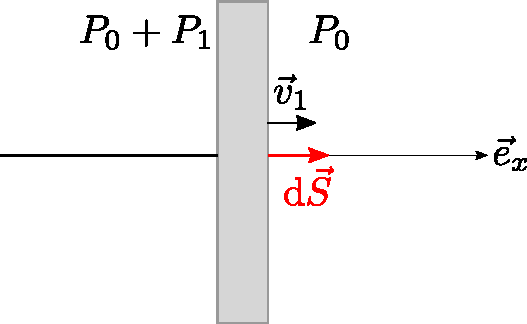
\includegraphics[width=0.37\textwidth]{Figures/paroi.pdf}
\caption{Surpression s'exerçant sur une paroi.}
\label{fig:paroi}
\end{figure}

Il s'ensuit que la puissance associée à cette force s'écrit $\d \mc{P}=p_1\vv{v_1}\cdot\vv{\d S}$. La puissance totale rayonnée par l'onde sonore se met donc sous la forme d'un flux
\begin{equation}
 \mc{P}=\iint_{S} p_1\vv{v_1} \cdot\vv{\d S}.
 \end{equation}
 On voit un apparaître un vecteur densité de courant d’énergie acoustique $\Vec{R} = p_1 \Vec{v_1}$.
\begin{definition}[Vecteur densité de courant d’énergie acoustique]\label{def:}
	Le vecteur \imp{densité de courant d’énergie acoustique} (en $ \SI{}{W.m^{-2}}$) s’écrit
$$
\Vec{R} = p_1 \Vec{v_1}.
$$
Le flux de $\Vec{R}$ sur une surface $S$ représente la puissance acoustique $\mc{P}$ traversant  $S$.
\end{definition}

% où nous avons défini le \important{vecteur de Poynting acoustique} homogène à une puissance par unité de surface, et donc exprimé en \SI{}{W.m^{-2}}.

\subsection{Équation de conservation de l’énergie acoustique}
% En électromagnétisme, nous avions obtenu une équation de conservation de l'énergie (plus précisément la puissance volumique) du champ électromagnétique sous la forme $\frac{\partial u_{\rm{em}}}{\partial t}+\dive{\,\vv{\Pi}}=-\vv{j}\cdot\vv{E}$, où $+\vv{j}\cdot\vv{E}$ désigne la puissance volumique cédée par le champ électromagnétique à la matière et $u_{\rm{em}}=\frac{1}{2}\varepsilon_0E^2+\frac{1}{2\mu_0}B^2$ désigne la densité volumique d'énergie du champ électromagnétique.
On souhaite obtenir une équation de conservation de l’énergie pour l'onde acoustique ? Celle-ci doit faire intervenir $\dive \Vec{R}$, par analogie avec $\dive \Poy$ en électromagnétisme.

Multiplions la première des équations \Eq{syst_couplé} par $v_1$ et la seconde par $p_1$,
\begin{equation}
\begin{subequations}
  \begin{cases}
  v_1\times(\rho_0\frac{\partial v_1}{\partial t}) = \frac{\partial }{\partial t}\left(\frac{1}{2}\rho_0 v_1^2\right)=-v_1\frac{\partial p_1}{\partial x}, \qquad \text{(Euler)}\\
    p_1\times(\chi_S\frac{\partial p_1}{\partial t}) = \frac{\partial }{\partial t}\left(\frac{1}{2}\chi_S p_1^2\right)=-p_1 \frac{\partial v_1}{\partial x}\qquad \text{(conservation de la masse)}\\
  \end{cases}
	\end{subequations}
  \end{equation}
	À présent, exprimons $\dive \Vec{R}$ pour voir comment faire apparaître ce terme. On a
\begin{equation}
	\dive \Vec{R} = \dive (p_1 v_1 \ex) = \dr{(p_1 v_1)}{x}  = p_1 \dr{v_1}{x} + v_1 \dr{p_1}{x}.
\end{equation}

  En prenant la somme des équations précédentes, on obtient donc
  \begin{equation}
  \frac{\partial}{\partial t}\left(\frac{1}{2}\rho_0 v_1^2+\frac{1}{2}\chi_S p_1^2\right)+\dive{\vv{R}}=0.
  \end{equation}
	On peut donc définir l'énergie acoustique par
	\begin{definition}[Densité volumique d'énergie acoustique]\label{def:}
		La densité volumique d'énergie acoustique (en $\SI{}{J.m^{-3}}$) s'écrit
		$$u_{a} = \frac{1}{2}\rho_0 v_1^2+\frac{1}{2}\chi_S p_1^2.$$
	\end{definition}

  La densité volumique d'énergie de l'onde acoustique se décompose en deux termes :
\begin{liste}
	\item densité volumique d'énergie cinétique de l'onde, $u_c = \frac{1}{2}\rho_0 v_1^2$ ;
	\item densité volumique d'énergie potentielle pressante, $u_p = \frac{1}{2}\chi_S p_1^2$. Les zones de forte pression correspondent en effet à des régions où les particules sont plus comprimés qu'ailleurs, c'est-à-dire une zone d'où les particules s'éloignent, en suivant la direction opposée au gradient de pression $-\grad p_1$.
\end{liste}
On remarque qu'il n'y a pas de terme de production volumique d'énergie acoustique.
\begin{theorem}[Équation de conservation de l’énergie acoustique]\label{form:}
$$
\dr{u_a}{t} + \dive \Vec{R} = 0.
$$
\end{theorem}

	 % d'une part la  et d'autre part une . La somme des deux, $e_{\rm{ac}}=\frac{1}{2}\chi_S p_1^2+\frac{1}{2}\rho_0 v_1^2$ désigne la densité volumique d'énergie de l'onde acoustique.

\subsection{Répartition d'énergie}
L'énergie du champ est-elle plutôt stockée dans la composante cinétique ou potentielle ? Cela dépend du type d'onde considéré, mais nous allons montrer que dans certains cas la relation entre les deux composantes de l'énergie acoustique est simple à exprimer.
\parag{OPP}
Considérons une onde plane progressive (OPP, pas nécessairement harmonique) se propageant selon les $x$ croissants. Alors $p_1=Zv_1=\sqrt{\frac{\rho_0}{\chi_S}}v_1$. Dans ce cas, on a
\begin{equation}
	u_{\rm p} = \frac{1}{2}\chi_S p_1^2 = \frac{1}{2}\chi_S\left(\frac{\rho_0}{\chi_S}\right)v_1^2 = \frac{1}{2}\rho_0v_1^2 = u_{\rm c}
\end{equation}
Les densités d'énergie potentielle et cinétique sont égales : on dit alors qu'il y a \important{équipartition} de la densité volumique d'énergie acoustique.

\begin{prop}[Équipartition de la densité d'énergie acoustique]\label{prop:}
	Dans une OPP acoustique, il y a \imp{équipartition} de la densité volumique d'énergie,
	$$
u_c  = u_p.
	$$
\end{prop}
La densité totale d'énergie vaut alors
\begin{equation}
u_{\rm{a}}=\rho_0 v_1^2=\chi_S p_1^2.
\end{equation}

\parag{OPPH}
Pour une OPPH, on a de plus $v_1=v_{\rm{m}}\cos(\omega t-kx + \vphi)$ si l'on chosit la direction de propagation comme étant $(Ox)$. La densité volumique d'énergie acoustique moyenne (calculée sur une période $T$) vaut alors
\begin{equation}
\moy{u_{\rm{a}}} = \frac{1}{T}\int_{0}^{T} e_a \d t = \frac{1}{T}\int_{0}^{T}\rho_0 v_1^2 \d t = \frac{1}{T}\int_{0}^{T}\rho_0 v_{\rm{m}}^2\cos^{2}(\omega t-kx + \vphi)\,\d t=\frac{\rho_0 v_{\rm{m}}^2}{2}.
\end{equation}

\begin{remarque}
Cette densité volumique d'énergie moyenne ne dépend plus des variables d'espace ! Par conséquent si on l'intègre dans tout l'espace on obtiendra une quantité infinie. Ceci illustre que le modèle de l'onde plane progressive harmonique n'est valable que \important{localement}.
\end{remarque}

On montre de la même façon le vecteur densité de courant d'énergie acoustique moyen vaut
\begin{equation}
\moy{\Vec{R}}=\frac{1}{T}\int_{0}^{T} p_1v_1 \ex \d t = \rho_0 c \,\frac{1}{T}\int_{0}^{T} v_{m}^2 \cos^{2}(\omega t-kx + \vphi)\d t\, \ex = c \,\frac{\rho_0 v_{m}^2}{2} \ex.
\end{equation}
On obtient alors une relation entre vecteur densité de courant et densité d'énergie,
\begin{equation}
	\moy{\Vec{{R}}}=c \moy{u_{\rm{a}}} \Vec{n},
\end{equation}
pour un direction de propagation quelconque $\Vec{n}$.
Cela indique que $c$ correspond physiquement à la vitesse de propagation de l'énergie de l'onde acoustique.
\begin{prop}[Vitesse de déplacement de l'énergie]\label{prop:}
	L'énergie acoustique se déplace à la célérité $c$ dans la direction de propagation $\Vec{n}$. Une OPPH vérifie
	$$
\moy{\Vec{R}}=c \moy{u_{\rm{a}}} \Vec{n}.
	$$
\end{prop}
%De plus, le vecteur de Poynting acoustique $\vv{\Pi}$ représente le vecteur densité de courant d'énergie acoustique. La valeur moyenne de sa norme,
% \begin{equation}
% I=\moy{\,||\vv{\Pi}||\,}
% \end{equation}
% représente l'intensité de l'onde sonore.

\parag{OPS} Pour une onde plane stationnaire (OPS), $v_1=v_{\rm{m}}\cos(\omega t)\cos(kx)$ et $p_1=\rho_0 c v_{\rm{m}}\sin(\omega t)\sin(kx)$ sont en quadrature de phase. Il vient alors qu'en moyenne
\begin{equation}
\moy{\Vec{R}}=\rho_0 c v_{1,\rm{m}}^2\cos(kx)\sin(kx)\moy{\cos(\omega t)\sin(\omega t)} \ex= \Vec{0}.
\end{equation}
\begin{prop}\label{prop:}
	En moyenne, une onde stationnaire ne transporte \imp{pas d'énergie}.
\end{prop}

\subsection{Intensité acoustique}

% \paragraph{Décibels acoustiques.\\}
La grandeur $\moy{R}$ représente la puissance surfacique transmise par l'onde. Or la sensibilité de l'oreille  est plutôt une fonction logarithmique de la puissance. On définit alors l'intensité acoustique exprimée en decibel (dB) comme
\begin{definition}[Intensité acoustique]\label{def:}
	On définit l'intensité sonore à partir de la puissance surfacique moyenne $\moy{R}$ par
	\begin{equation*}
	I (\text{en dB})=10\,\log\left(\frac{\moy{R}}{R_{\rm ref}}\right),
\end{equation*}
où $R_{\rm ref} = \SI{e-12}{W.m^{-2}}$ représente la plus petite puissance surfacique sonore que l'oreille perçoit.
\end{definition}

La grandeur $R_{\rm ref}$ représente la puissance acoustique minimale que l'oreille humaine est capable de percevoir. Sachant que $R \propto p_1^2$, on peut aussi écrire l'intensité acoustique sous la forme
% \begin{equation}
	\eqbox[]{
		I=20\,\log\left(\frac{p_1}{p_{\rm{ref}}}\right)\quad\text{en dB}.
	}
% \end{equation}
% En réalité le bel n'est jamais employé comme unité et on lui préfère le décibel (dB) de sorte que
où $p_{\rm{ref}}=\SI{20}{\micro Pa}$ la pression de référence ; il s'agit de la pression minimale audible. Quelques ODG d'intensité acoustique sont donnés \Fig{echelle}.
%
% \begin{exemple}{Ordres de grandeurs d'intensités acoustiques}
% 	Dans le cas de l'exemple précédent de l'enceinte, on obtient une intensité sonore de $\SI{120}{dB}$ ce qui est très important (typiquement l'intensité sonore d'une boite de nuit). \SI{20}{dB} correspond à des chuchotements, \SI{60}{dB} le bruit d'une conversation normale, \SI{80}{dB} le bruit du traffic routier en ville. Au dessus de \SI{120}{dB}, c'est le seuil de douleur. Rappelons enfin que doubler l'intensité sonore revient à ajouter \SI{3}{dB} (car $10\log(2)\simeq 3$), diviser l'intensité sonore par deux revient à enlever \SI{3}{dB}.
\begin{figure}[H]
	\centering
	
\includegraphics[width=0.6\textwidth]{Echelle-sonore.png}
	\caption{Échelle d'intensité acoustique.}
	\label{fig:echelle}
\end{figure}
% \end{exemple}




\begin{exemple}{Validation de l'approximation acoustique}
	Une personne écoute de la musique d'une enceinte bluetooth portable de puissance acoustique $\mc{P}=\SI{1}{W}$ placée à une distance $d=\SI{1}{m}$.  Dans l'air, $\rho_0\simeq\SI{1,2}{kg.m^{-3}}$
	et $c\simeq\SI{340}{m.s^{-1}}$. On donne $p_{\rm{ref}}=\SI{20}{\micro Pa}$ la pression de référence pour le calcul de l'intensité sonore.
	\begin{quest}
		\item Déterminer la puissance surfacique rayonnée par l'enceinte à la distance $d$.
		\item En déduire l'amplitude de la vitesse particulaire $v_1$.
		\item En déduire la surpression acoustique $p_1$ et l'intensité sonore $I$.
	\end{quest}
\end{exemple}
\examplesol{
	\begin{quest}
		\item La puissance surfacique rayonnée vaut 
		\eqbox{
		R = \mc{P}/4\pi d^2 =  \SI{8e-2}{W.m^{-2}}. 
			}
		\item On sait que $R = \frac{1}{2}\rho_0 c v_{\rm{m}}^2$ pour une OPPH, ce qui donne 
		\eqbox{
			v_{\rm{m}}\simeq\SI{6}{cm.s^{-1}}.
		}
		Cette valeur est très petite devant la vitesse du son : $v_1\ll c$, ce qui justifie l'approximation acoustique.
	\item 
		De plus, on trouve $p_1=\rho_0 c v_{\rm{m}}\simeq \SI{25}{Pa}$, qui est très petite devant $p_0 \simeq \SI{1}{bar}=\SI{e5}{Pa}$, validant à nouveau l'approximation acoustique. Cette pression correspond à une intensité sonore
		\eqbox{
			I= 20 \log\left(\frac{p_1}{p_{\rm ref}}\right) \simeq \SI{120}{dB}.
		}
	\end{quest}
}

\subsection{Analyse énergétique d'une onde sphérique}
Le vecteur densité de courant d'énergie acoustique s'écrit pour une onde divergente
\begin{equation}
	\Vec{R} = p_1 \Vec{v_1} = \frac{A}{r}\cos(\omega t-kr+\varphi) \frac{\underline{A}}{\rho_0 c}\left(\frac{\cos(\omega t-kr)}{r}+\frac{\sin(\omega t-kr)}{kr^2}\right)\vv{e_r}.
\end{equation}
En moyennant sur le temps, seule la composante en phase (champ lointain) contribue,
\begin{equation}
	\moy{\Vec{R}} = \frac{A^2}{2\rho_0 c r^2} \er.
\end{equation}
La puissance acoustique traversant une sphère centrée en $O$ de rayon $r$ vaut alors
\begin{equation}
	\mc{P} = \iint_S \moy{\Vec{R}} \ps \dS = \frac{A^2}{2\rho_0 c r^2}\times (4\pi r^2) = \frac{2 \pi A^2}{\rho_0 c}.
\end{equation}
Cette puissance ne dépend pas de $r$, ce qui traduit la conservation de l'énergie. La décroissance de l'amplitude en $1/r$ assure cette conservation.


\end{document}
